\documentclass[11pt]{article}
\usepackage{tikz}
\usepackage{pgfplots}
\usepackage{graphicx}
\usepackage{amsmath}
\usepackage{amssymb}

\pgfplotsset{compat=1.18}

\usetikzlibrary{shapes.geometric, arrows}
\tikzstyle{item} = [rectangle, rounded corners, minimum width=3cm, minimum height=1cm,text centered, draw=black, fill=red!30]\tikzstyle{arrow} = [thick,->,>=stealth]

% Margins
\topmargin=-0.45in
\evensidemargin=0in
\oddsidemargin=0in
\textwidth=6.5in
\textheight=9.0in
\headsep=0.25in

\title{
	\centering
	\includegraphics[width=5cm]{univ-logo} \\
	\vspace{5cm}
	\textbf{SAT solvers} \\
	Computational Models of Argumentation
	\vspace{5cm}
}
\author{
    Christophe Yang \\
    Quentin Januel \\
    Sylvain Declercq
}
\date{2022}

\begin{document}

\maketitle
\newpage

\tableofcontents
\newpage

\section{Flowchart}
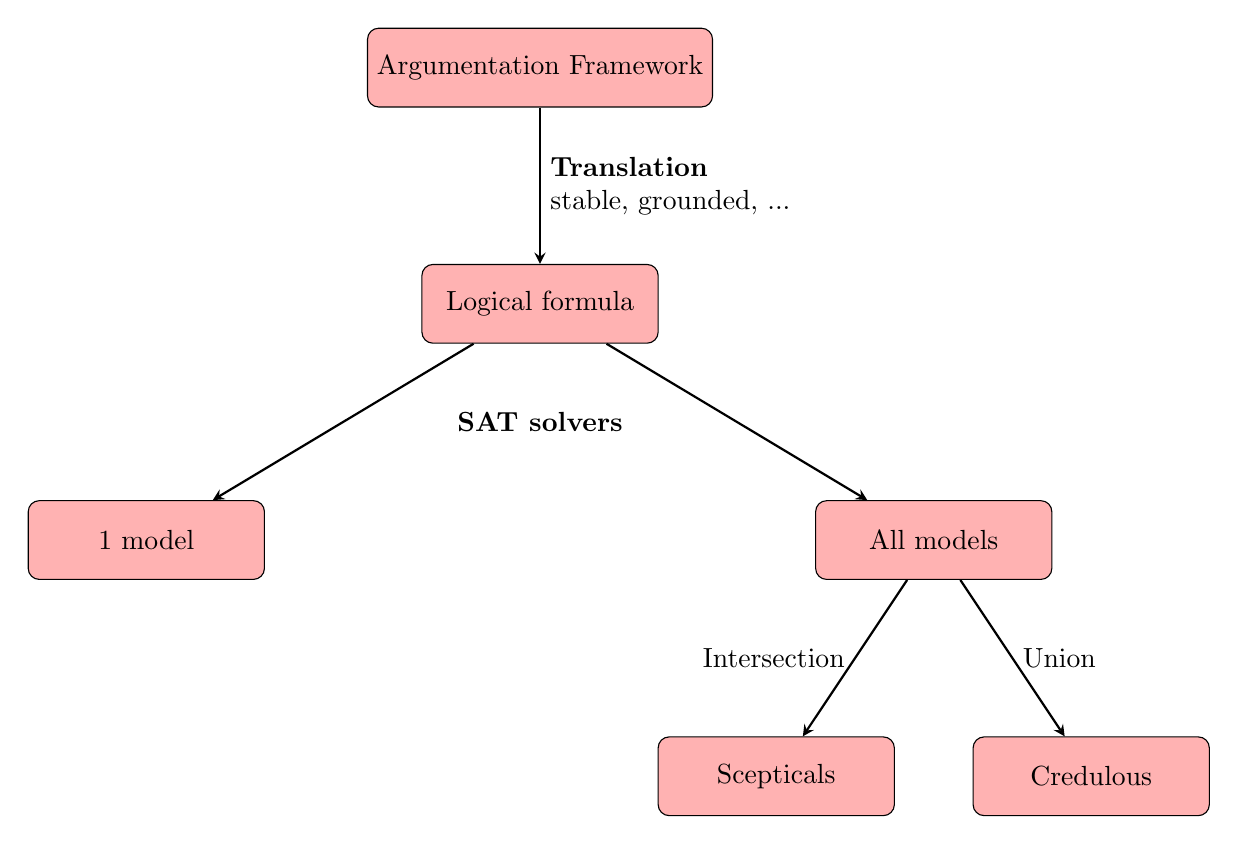
\begin{tikzpicture}[node distance=3cm]
\node(af)[item]{Argumentation Framework};
\node(log)[item, below of=af]{Logical formula};
\draw[arrow] (af) -- node[anchor=west, text width=4cm]{\textbf{Translation}\\stable, grounded, ...} (log);
\node(sat1)[item, below of=log, xshift=-5cm]{1 model};
\node(satall)[item, below of=log, xshift=5cm]{All models};
\node[below of=log, yshift=1.5cm]{\textbf{SAT solvers}};
\draw[arrow] (log) -- (sat1);
\draw[arrow] (log) -- (satall);
\node(scept)[item, below of=satall, xshift=-2cm]{Scepticals};
\node(cred)[item, below of=satall, xshift=2cm]{Credulous};
\draw[arrow] (satall) -- node[anchor=east]{Intersection} (scept);
\draw[arrow] (satall) -- node[anchor=west]{Union} (cred);
\end{tikzpicture}
\newpage

\section{Extensions}
Let $F := (A, R)$ be an Argumentation Framework and $S \subset A$, then $S$ is
\begin{itemize}

\item \textbf{conflict-free} if for all $(a, b)$ in $S^2$, $(a, b)$ is not in $R$.
$$
\phi_{cf}(F) = \bigwedge_{(a, b) \in R} \lnot a \lor \lnot b
$$
\item \textbf{admissible} if $S$ is conflict-free and defends all its arguments.
$$
\phi_{ad}(F) = \phi_{cf}(F) \land \bigwedge_{a \in A} \left( a \implies \bigwedge_{(b, a) \in R} \bigvee_{(c, b) \in R} c \right)
$$
\item \textbf{complete} if $S$ is admissible and contains all the arguments that it defends.
$$
\phi_{co}(F) = \phi_{cf}(F) \land \bigwedge_{a \in A} \left( a \iff \bigwedge_{(b, a) \in R} \bigvee_{(c, b) \in R} c \right)
$$
\item \textbf{grounded} if $S$ is complete and that there is no complete extension $S' \neq S$ such that $S' \subset S$.
Apply unit propagation to $\phi_{co}$.
\item \textbf{preferred} if $S$ is complete and that there is no complete extension $S' \neq S$ such that $S \subset S'$.
There is no encoding to SAT. Instead, use $\phi_{co}$ and if the solution is not preferred, forbid it in the logical formula and try again.
\item \textbf{stable} if $S$ is conflict-free and attacks all the arguments it does not contain.
$$
\phi_{st}(F) = \bigwedge_{a \in A}\left(a \iff \bigwedge_{(b, a)\in R} \lnot b\right)
$$

\newpage
\section{Schema}
In the schema below, the arrow is an implication. \\ \\
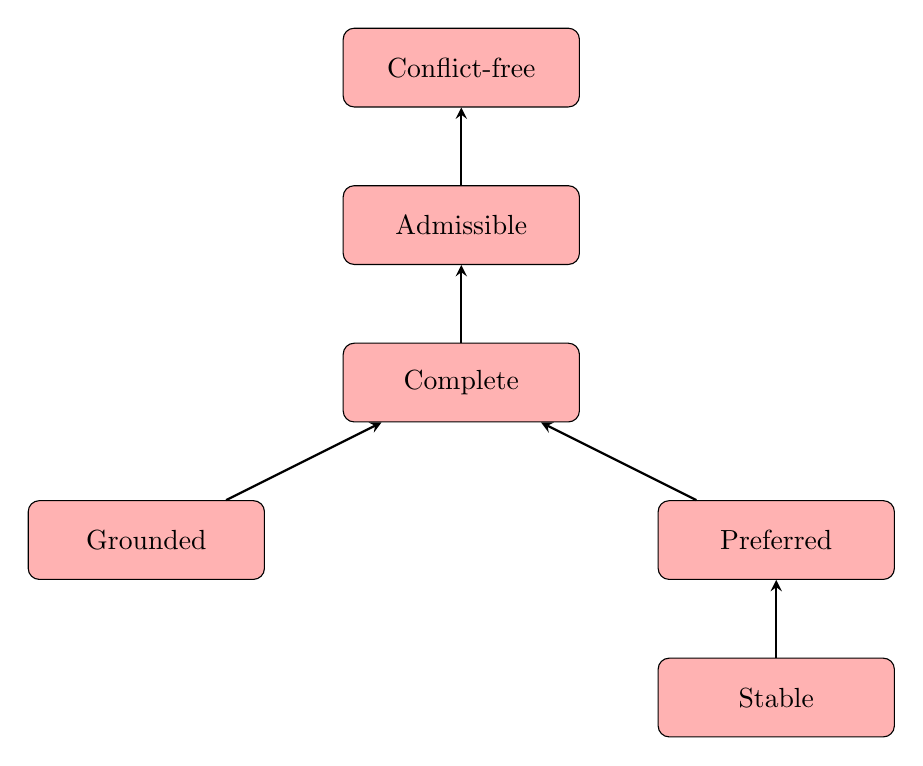
\begin{tikzpicture}[node distance=2cm]
\node(cf)[item]{Conflict-free};
\node(adm)[item, below of=cf]{Admissible};
\draw[arrow] (adm) -- (cf);
\node(comp)[item, below of=adm]{Complete};
\draw[arrow] (comp) -- (adm);
\node(grounded)[item, below of=comp, xshift=-4cm]{Grounded};
\node(preferred)[item, below of=comp, xshift=4cm]{Preferred};
\draw[arrow] (grounded) -- (comp);
\draw[arrow] (preferred) -- (comp);
\node(stable)[item, below of=preferred]{Stable};
\draw[arrow] (stable) -- (preferred);
\end{tikzpicture}

\end{itemize}


\end{document}
